\subsection{Statistical Analysis}
\label{sec:statistical-analysis}

This section presents the statistical analysis of the results of the study.
We employ a systematic approach to compare the performance of different models and their configurations.

\textbf{Note:} In order to keep the tables and figures reasonable in size, we use a short label system
for model configurations. The legend for these labels can be found in the appendix \autoref{sec:appendix}.

\subsubsection*{Tests Considered}
There are various statistical tests available to compare the performance of machine learning models.
We considered the following tests for our analysis:

\subsubsection{ANOVA}
Analysis of Variance (ANOVA) decomposes the total variance in the data into different components such as:
between-classifier variability, between-dataset variability, and residual variability. When between-classifier
variability is significantly larger than the residual variability, we can reject the theorised null hypothesis and
conclude that there is a significant difference between the classifiers.

However, ANOVA assumes that the data is drawn from normal distributions and that the variances are equal across groups.
In the case of the hepatitis dataset, the class distribution is skewed (79 $-$ 21 split) \cite{StatisticalComparisonsOfClassifiersOverMultipleDataSetsJML,Friedman_anova}.

\begin{figure}[!ht]
    \centering
    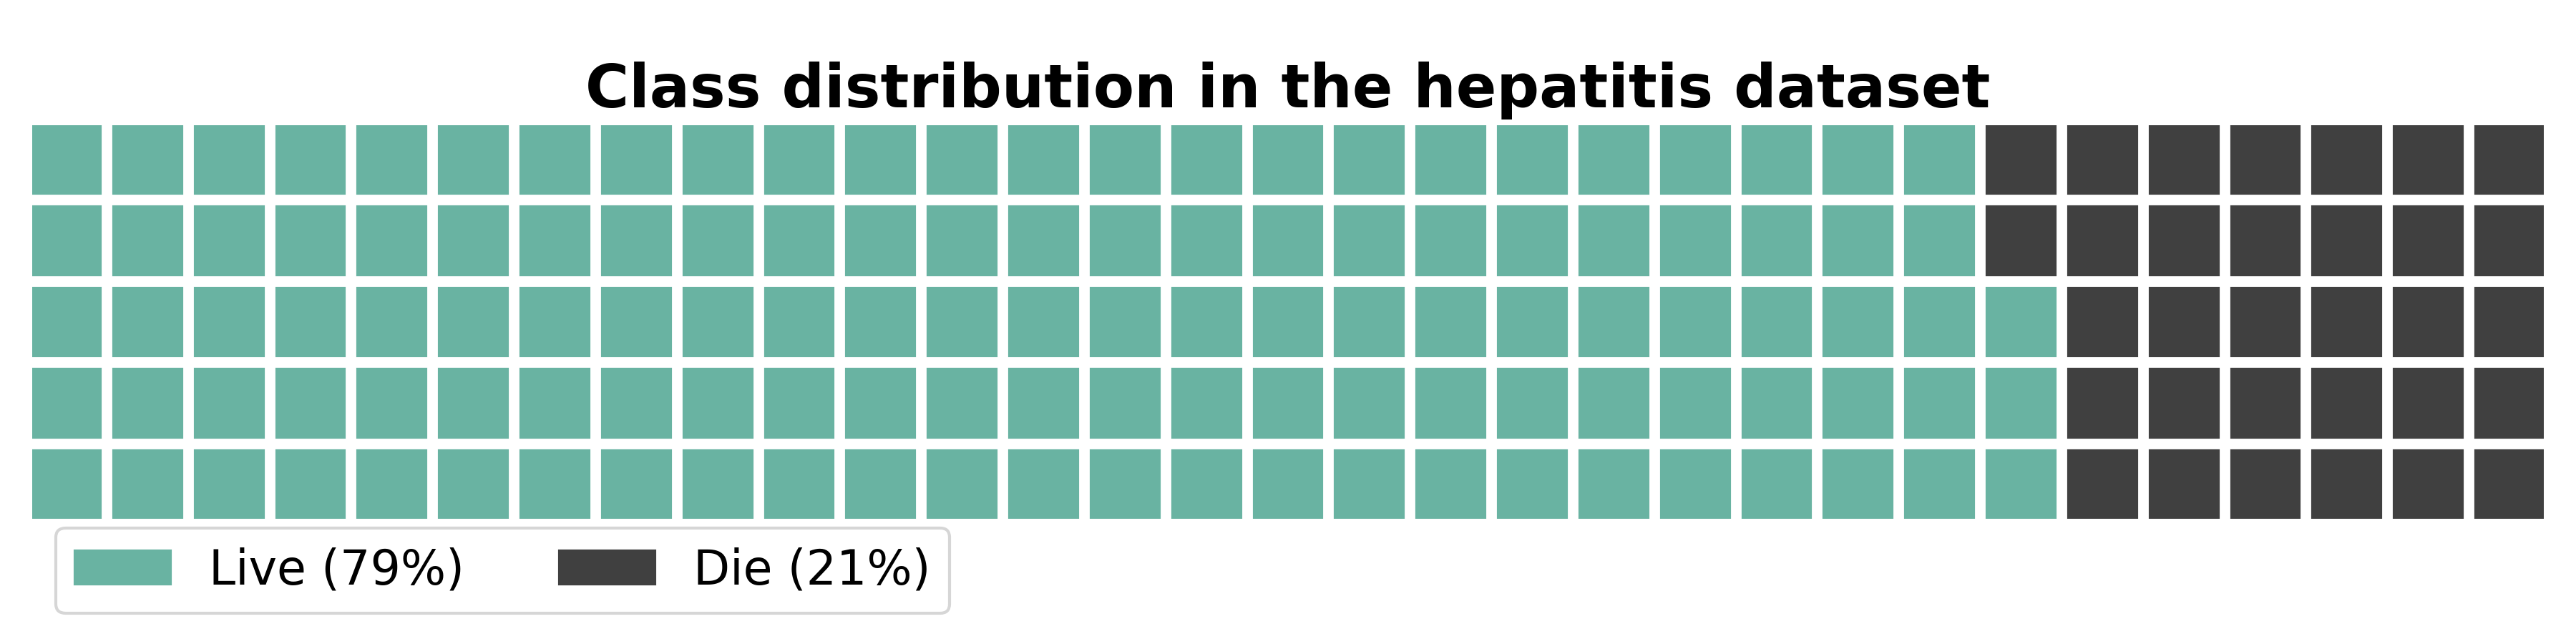
\includegraphics[width=0.9\textwidth]{figures/hepatitis-class-distribution.png}
    \caption{Class distribution of the Hepatitis dataset}
\label{fig:class-distribution-hepatitis}
\end{figure}

Furthermore, the performance metrics distribution across folds in Figure~\ref{fig:ranked-folds-knn-hepatitis} further demonstrates non-normal distribution:

\begin{figure}[!ht]
    \centering
    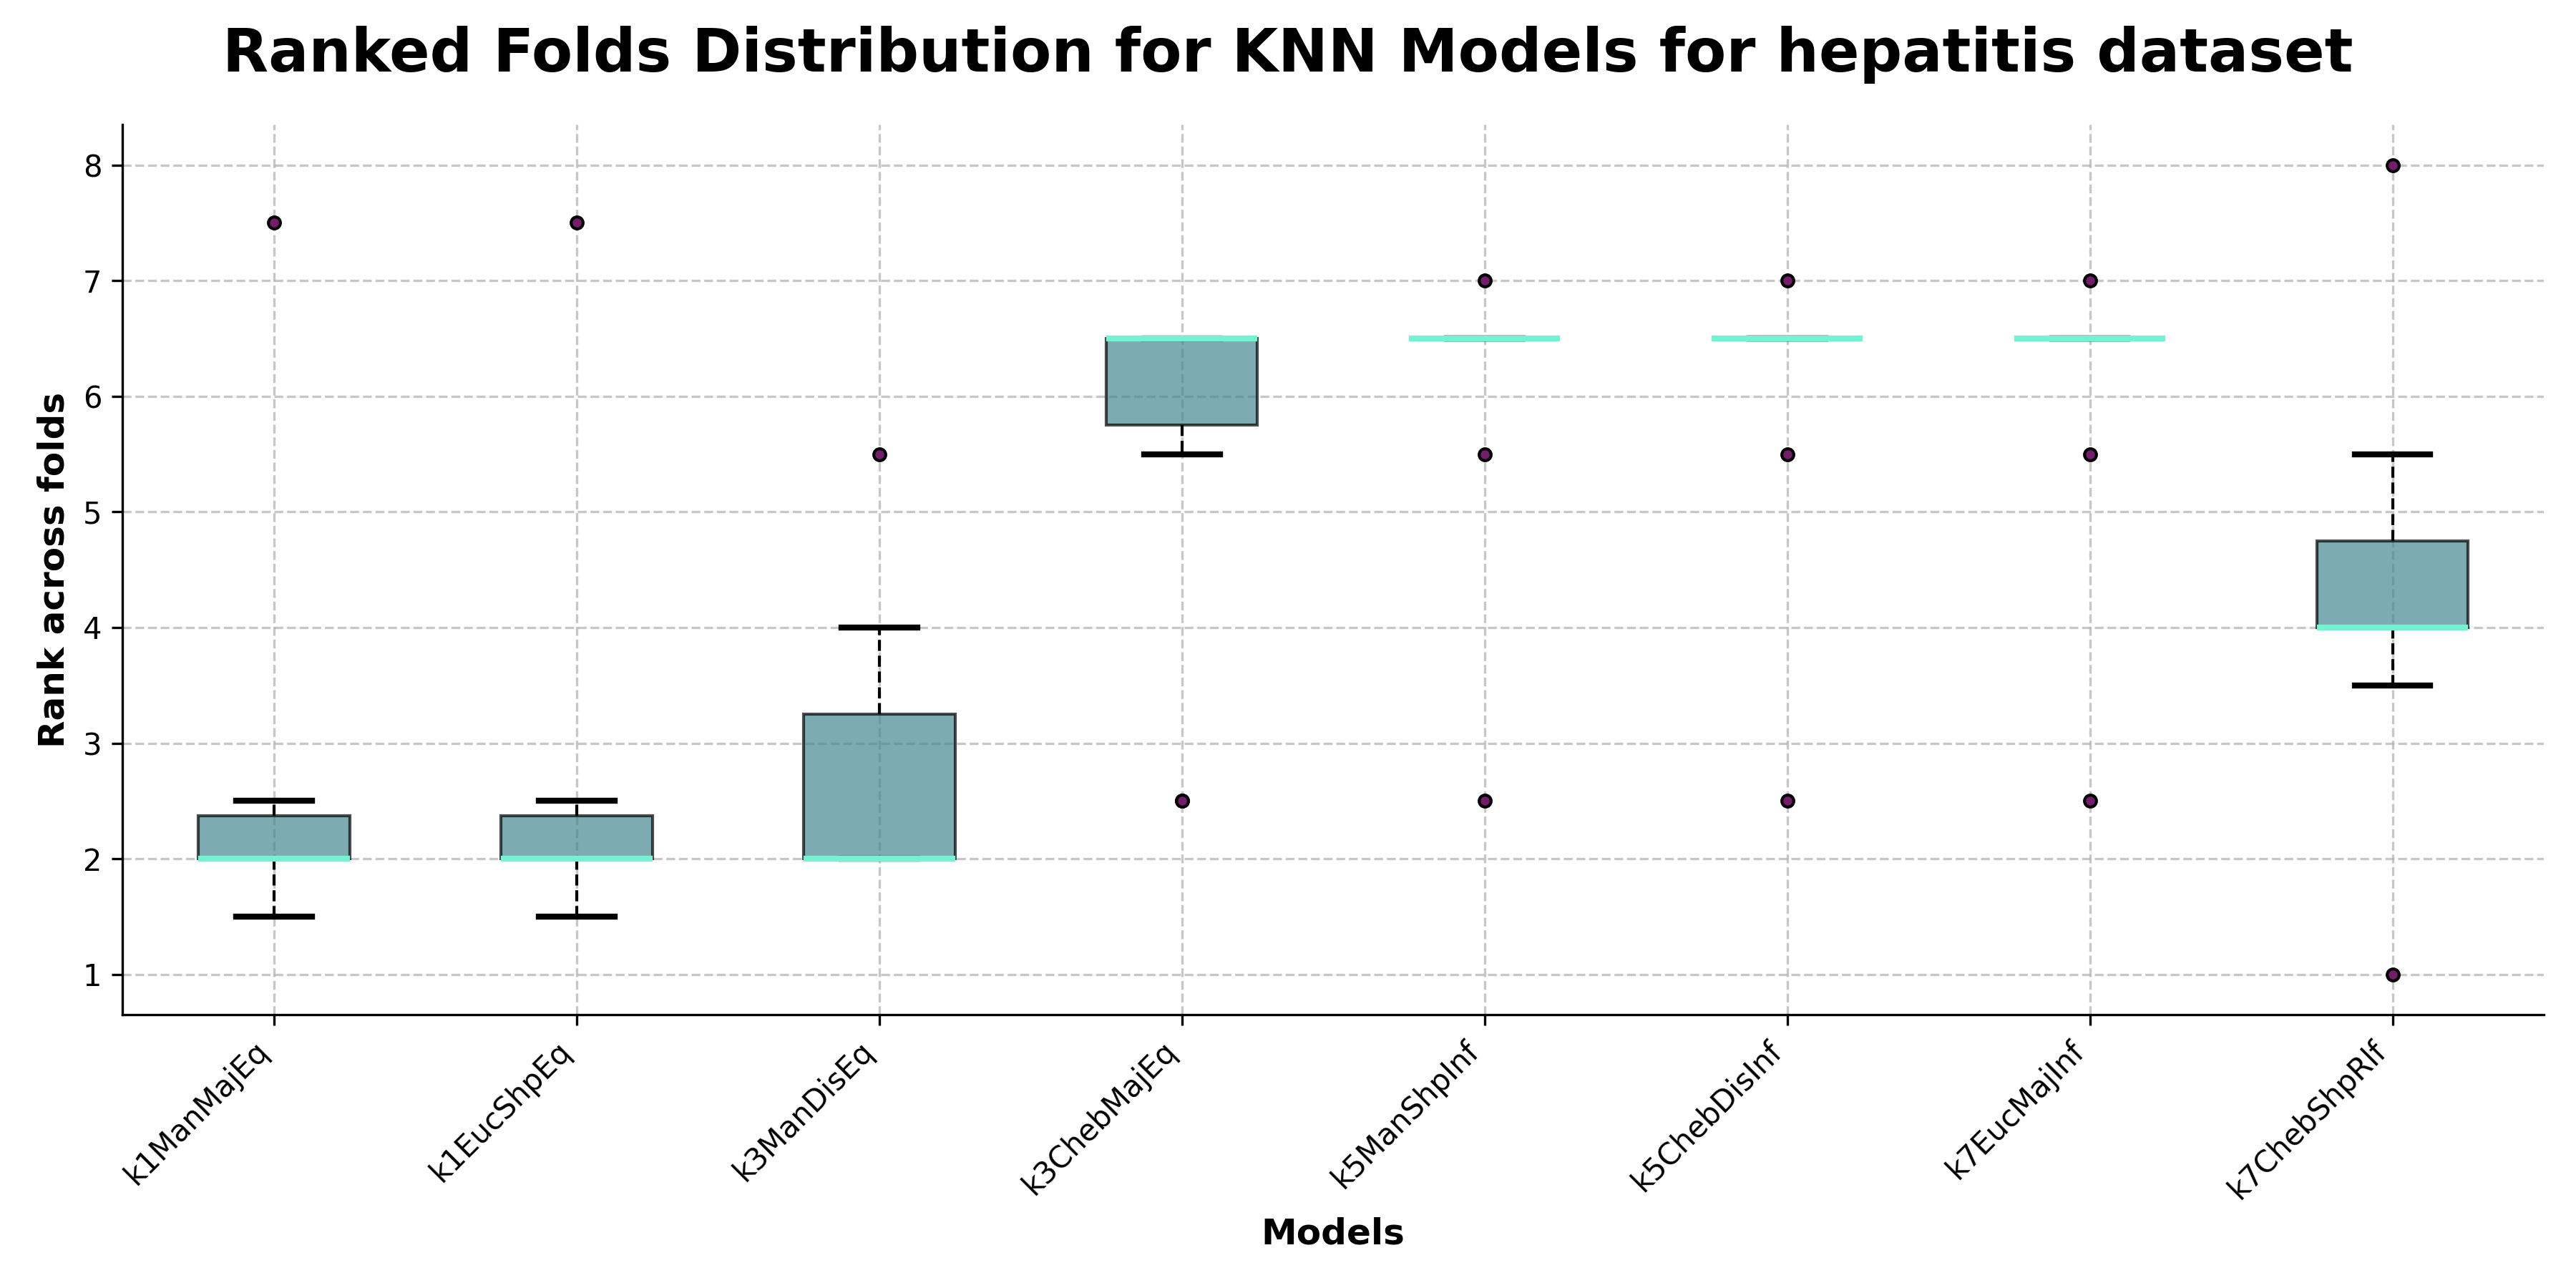
\includegraphics[width=0.9\textwidth]{figures/ranked_folds_KNN_hepatitis.png}
    \caption{Rank distributions across folds for different KNN configurations on the Hepatitis dataset}
\label{fig:ranked-folds-knn-hepatitis}
\end{figure}

These plots verify that the data does not meet the assumptions of ANOVA:

- Non-normal distribution: Several models show asymmetric distributions, where the median line is not in the middle of the box.
Also present are outliers in the data, which are represented as dots outside of the whisker lines.
- Unequal variances: Box sizes vary significantly across models, and some models have much larger spreads than others.
Additionally, the whisker lenghts vary considerably between models.

These claims hold true when analysing performance metrics distribution across folds using SVM:

\begin{figure}[!ht]
    \centering
    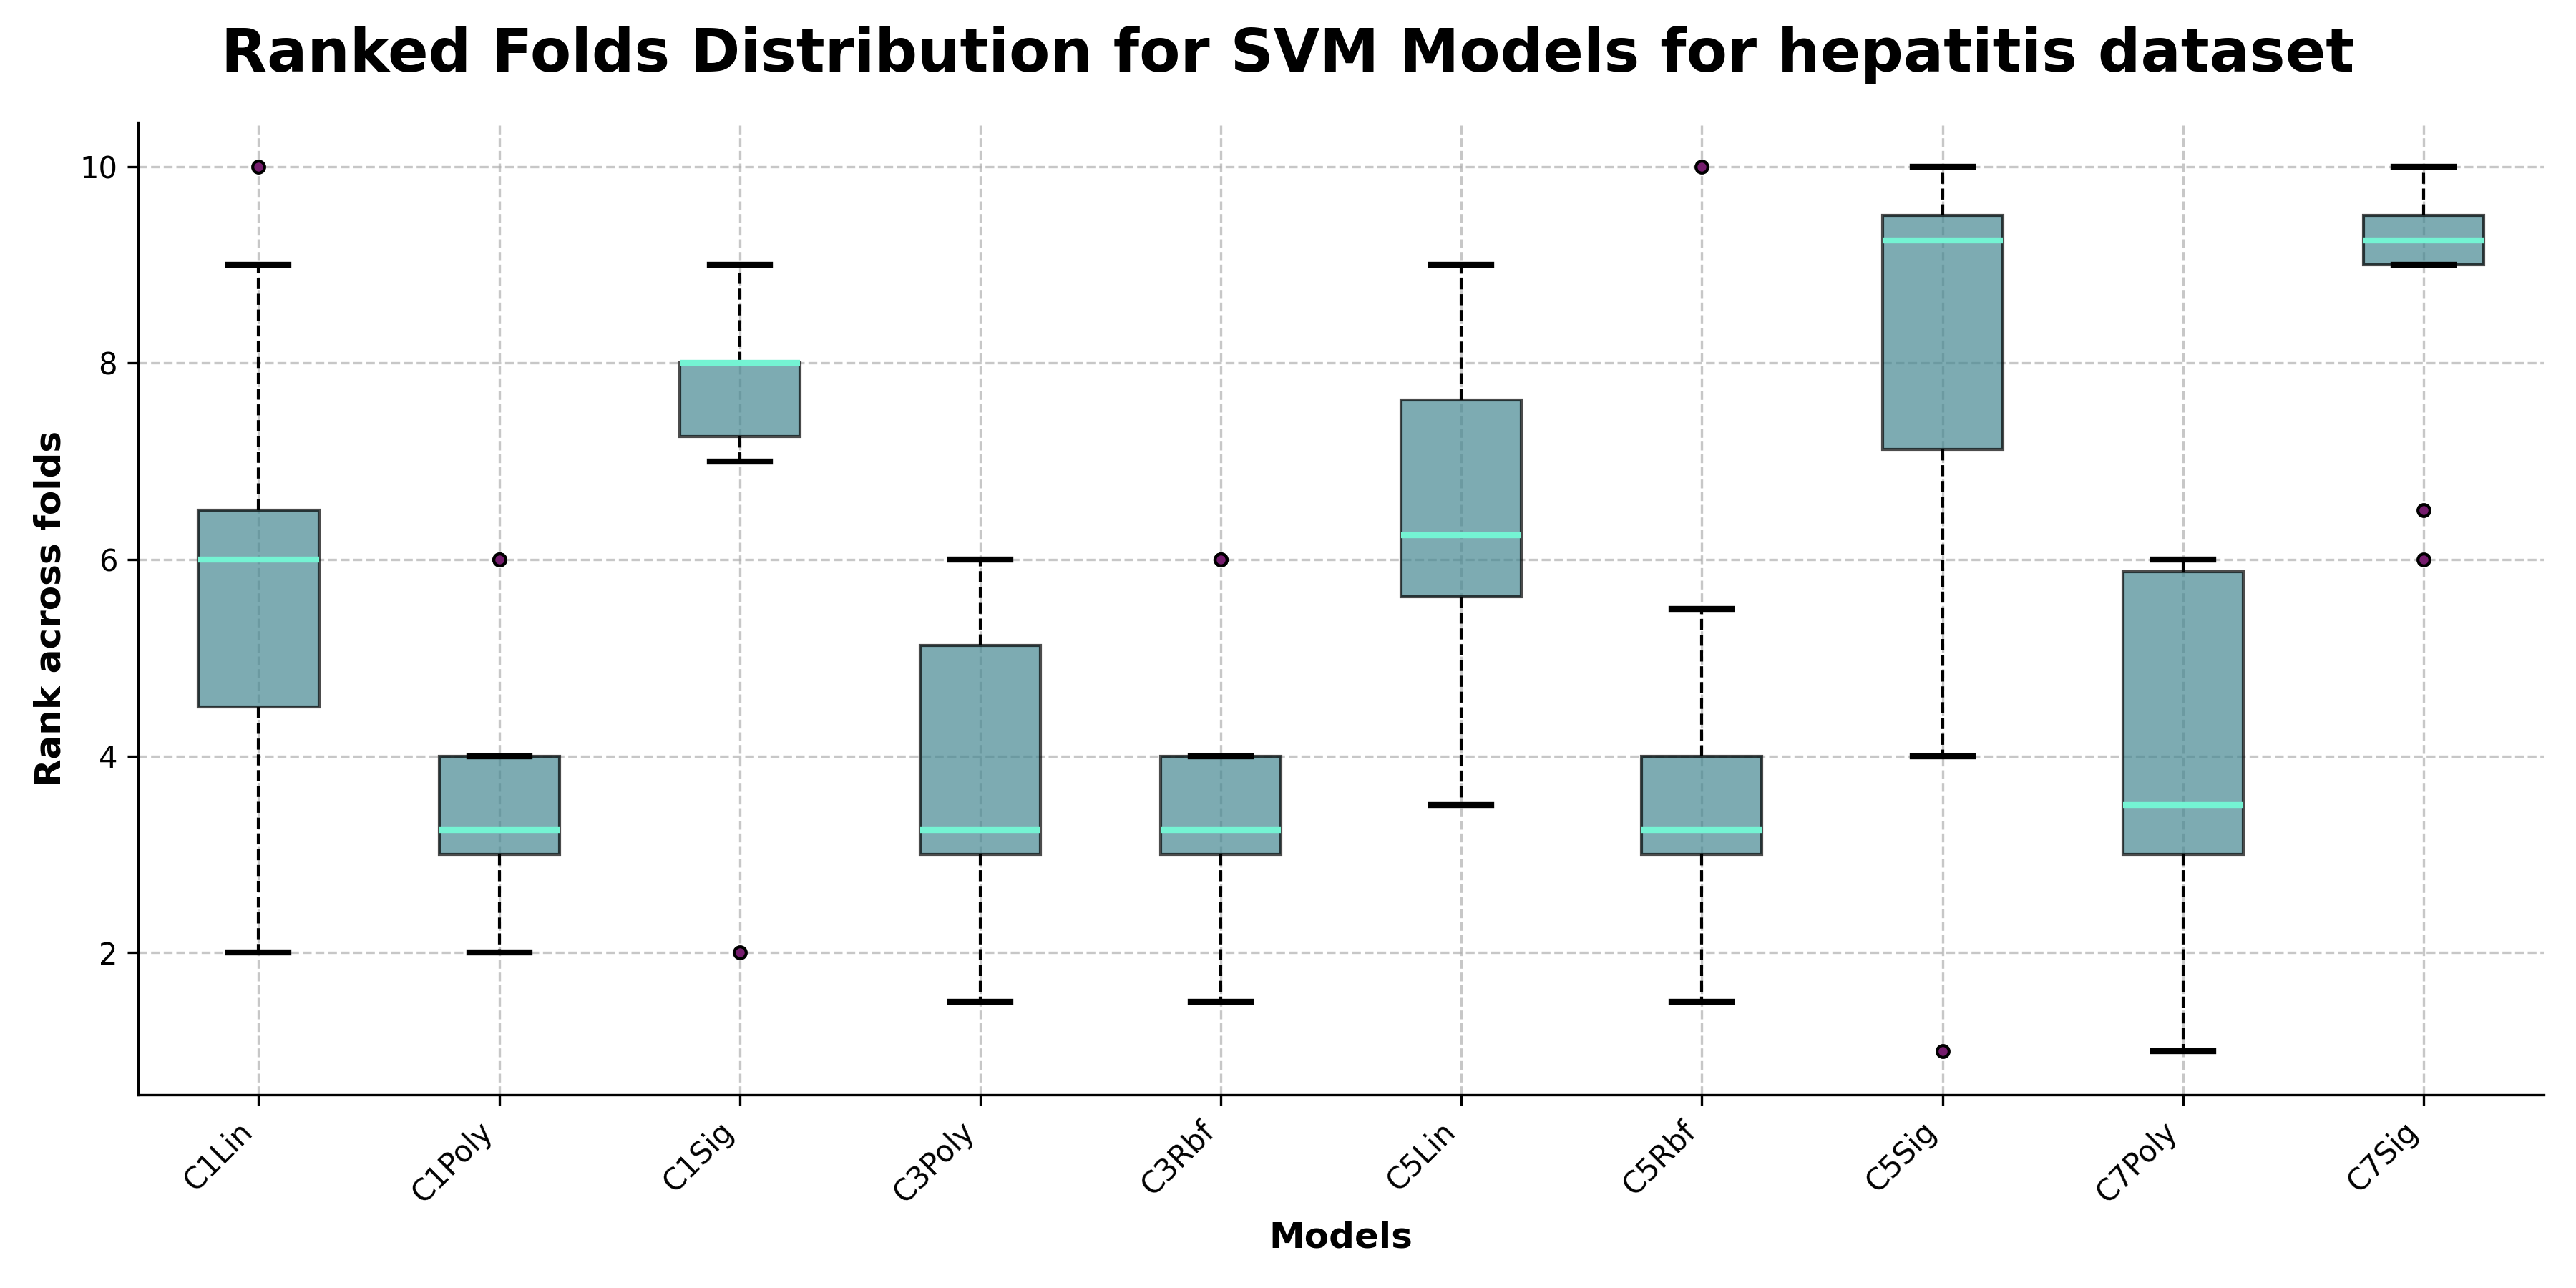
\includegraphics[width=0.9\textwidth]{figures/ranked_folds_SVM_hepatitis.png}
    \caption{Rank distributions across folds for different SVM configurations on the Hepatitis dataset}
\label{fig:ranked-folds-svm-hepatitis}
\end{figure}

Given these observations, we decided against using ANOVA for our analysis.

\subsubsection{Friedman Test}
The Friedman test is a non-parametric equivalent of the repeated-measures ANOVA. 
For each dataset, it ranks the models separately with the best model receiving a rank of 1, the second-best a rank of 2, and so on.
The average rank is used to settle any ties in the ranks \cite{Friedman_anova,Friedman_posthoc}.

While the Friedman test theoretically has less statistical power than ANOVA when ANOVA's assumptions are met,
it is more suitable for our analysis as it makes no assumptions about normality or equal variances.
As we demonstrated with the hepatitis dataset's class distribution and performance metrics, these assumptions do not hold in our case.

\subsubsection{Post-Hoc Testing}
The Friedman test only tells us that there is a significant difference between the models,
but it does not tell us which models are significantly different from each other.
This is why we employ the Nemenyi test as a post-hoc procedure.

The Nemenyi test compares the performance of all classifiers to each
other by checking if their average ranks differ by at least the critical difference:

\begin{equation}
    CD = q_{\alpha} \times \sqrt{\frac{k(k+1)}{6N}}
\end{equation}

where $q_{\alpha}$ is based on the Studentized range statistic, $k$ is the number of classifiers, and $N$ is
the number of datasets \cite{Friedman_posthoc}.
If the difference in average ranks between two models exceeds this critical difference, we can conclude that their performances are significantly different.

When performing the Nemenyi test, proper handling of ties is crucial for accurate analysis.
Instead of arbitrarily assigning consecutive ranks to tied values (e.g., ranks 2 and 3), we use the
average of the ranks they would have occupied. For example, if two models tie for second place,
rather than arbitrarily assigning ranks 2 and 3, both models receive a rank of 2.5 (the average of positions 2 and 3).
This mid-rank approach ensures fair treatment of tied performances and prevents artificial rank differences that could bias the statistical analysis.

In the visualisation of critical difference (CD) diagrams, the entire bar represents the critical difference value.
The half-width of the bar (CD/2) extends on either side of a model's average rank. When comparing two models,
if their CD/2 intervals do not overlap, we can conclude that there is a statistically significant difference in their performance.
This visual representation provides an intuitive way to interpret the Nemenyi test results, as any
non-overlapping bars clearly indicate significant differences between models.

\subsubsection{Linear vs. Top Sampling Justification}
The results of the Nemenyi test must satisfy the requirements to perform post-hoc testing.
If the Nemenyi test fails, we cannot proceed with post-hoc testing as the results would be considered unreliable.

\begin{figure}[!ht]
    \centering
    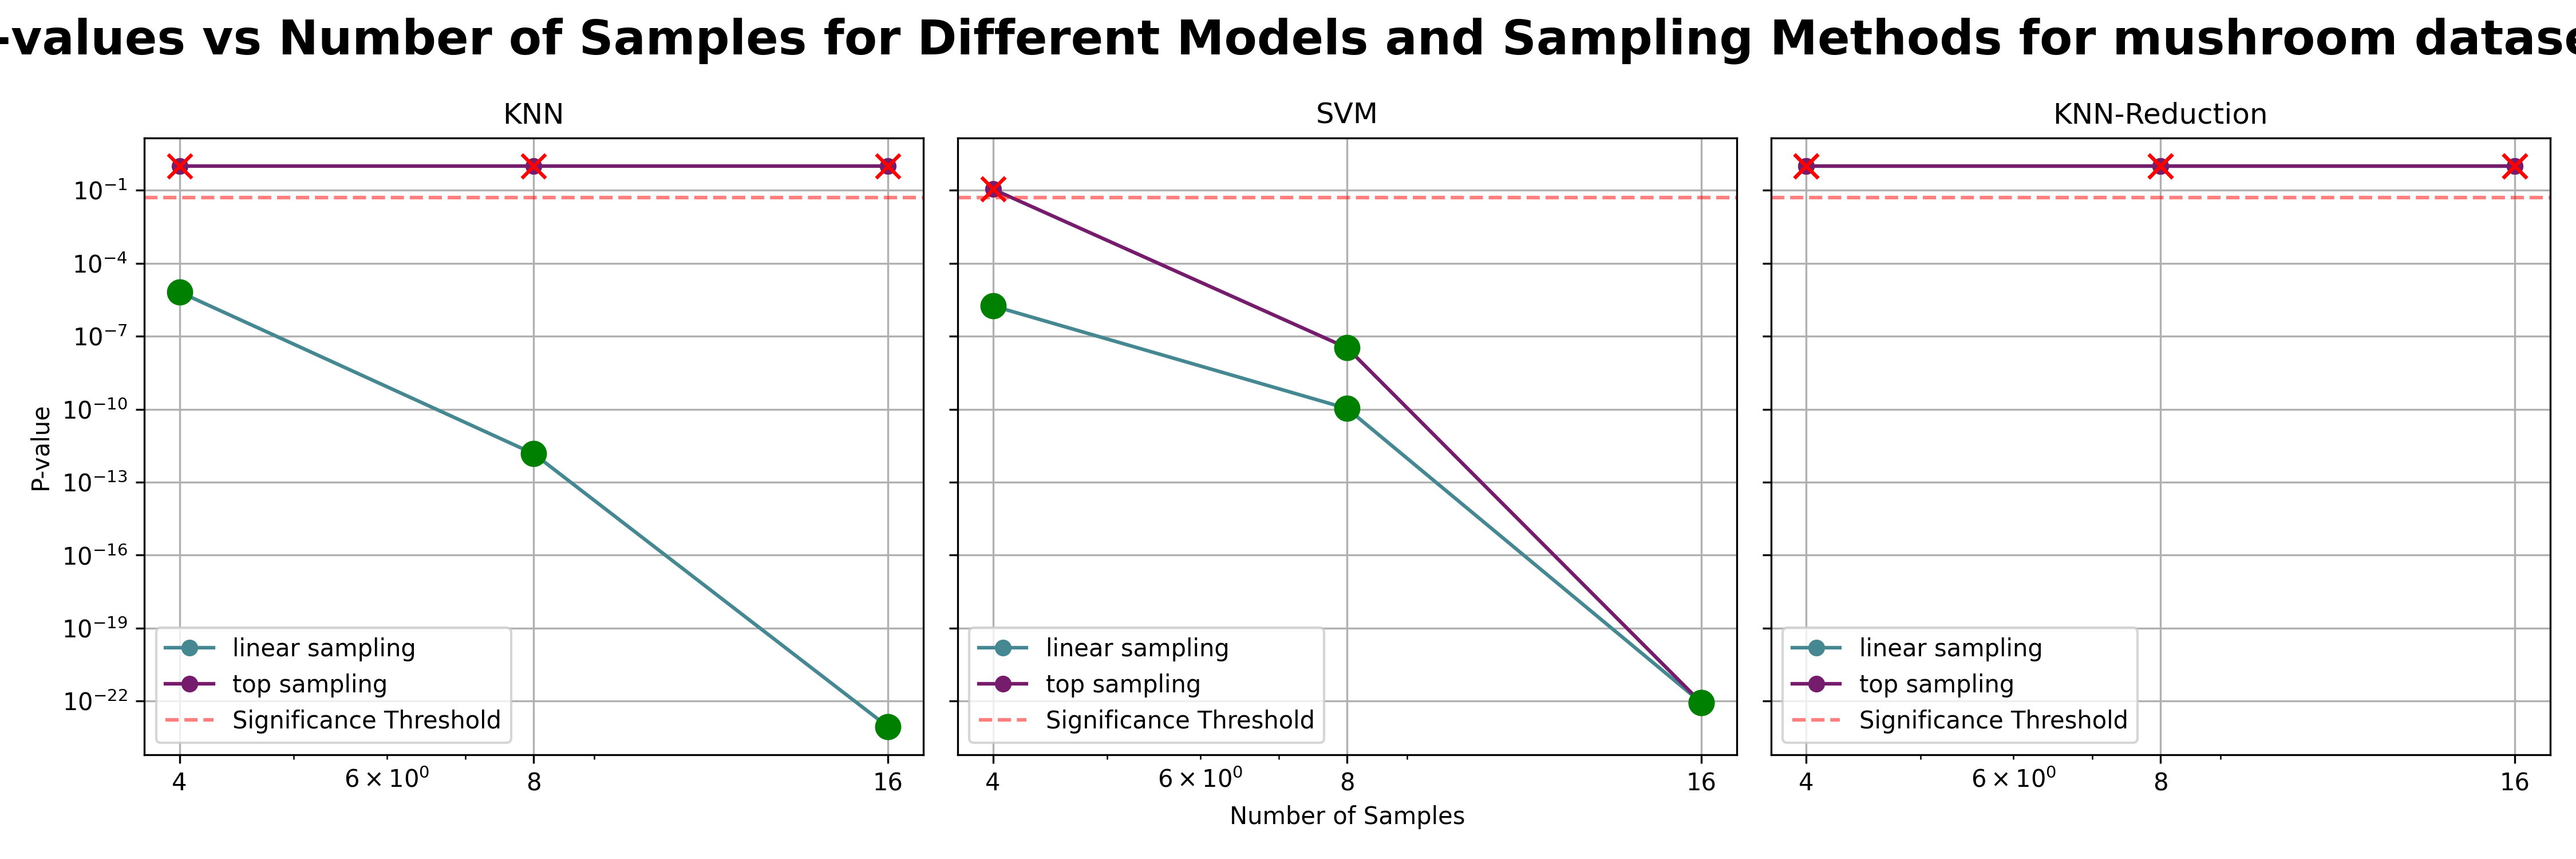
\includegraphics[width=0.8\textwidth]{figures/p_values_vs_num_samples_mushroom.png}
    \caption{P values vs. number of samples for different models and sampling methods for the datasets}
\label{fig:p_values_vs_num_samples_mushroom}
\end{figure}

\begin{figure}[!ht]
    \centering
    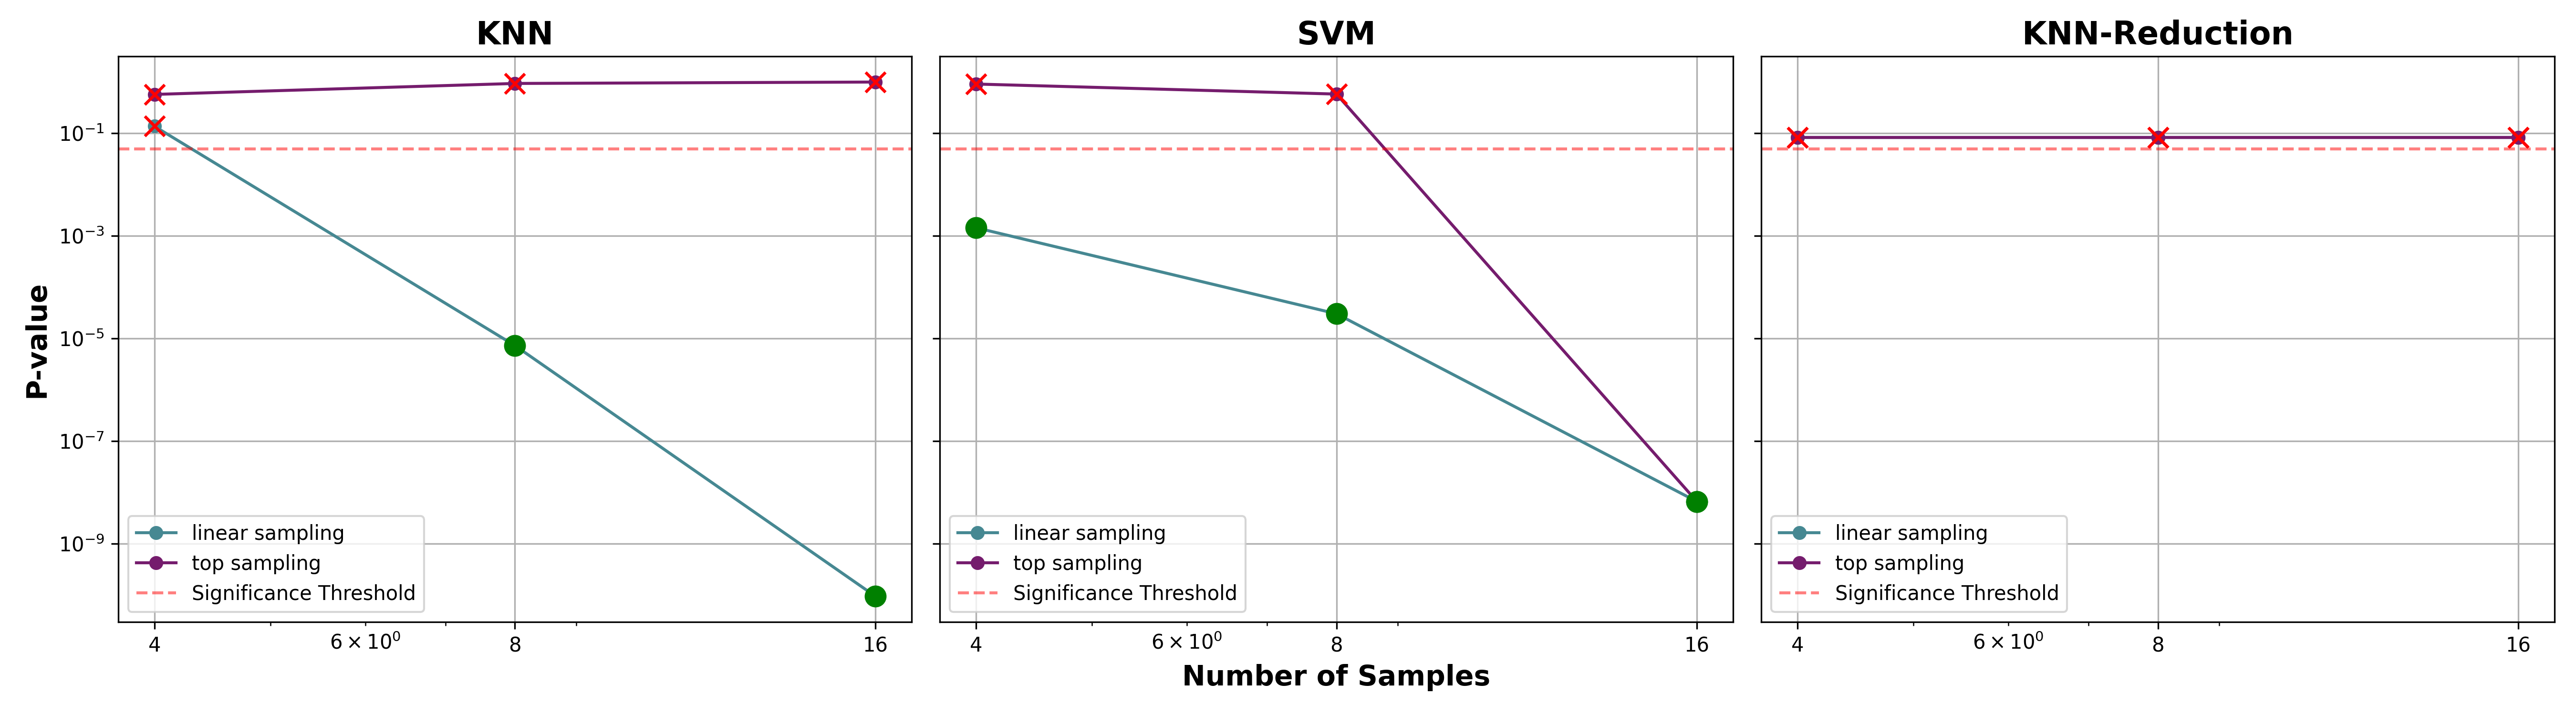
\includegraphics[width=0.8\textwidth]{figures/p_values_vs_num_samples_hepatitis.png}
    \caption{P values vs. number of samples for different models and sampling methods for the datasets}
\label{fig:p_values_vs_num_samples_hepatitis}
\end{figure}

As seen in \autoref{fig:p_values_vs_num_samples_mushroom} and \autoref{fig:p_values_vs_num_samples_hepatitis}, we perform linear sampling and top sampling with a variety
of sample sizes. With top sampling, we sample the top models based on their f1 score, while linear sampling samples models
evenly across the performance spectrum. The results show that the Nemenyi test fails across the various sample sizes for both datasets
when using top sampling but passes when using linear sampling.This indicates that the top sampling method is not suitable for our analysis
as we cannot perform post-hoc testing on the models.

To further justify our decision, see \autoref{tab:friedman_test_results_mushroom} and \autoref{tab:friedman_test_results_hepatitis} for the Friedman test results for both datasets.

\begin{table}
\centering
\caption{Friedman Test Results}
\label{tab:friedman_test_results_mushroom}
\begin{tabular}{ll}
\toprule
name & P Value \\
\midrule
KNN Top Sample of 8 F1 Scores & 1 \\
SVM Top Sample of 8 F1 Scores & 3.331542319440828e-08 \\
KNN Linear Sample of 8 F1 Scores & 1.477429493282523e-12 \\
SVM Linear Sample of 8 F1 Scores & 1.068518136588972e-10 \\
KNN-Reduction Linear Sample of 8 F1 Scores & 1 \\
SVM-Reduction Linear Sample of 8 F1 Scores & 1.3800570312932555e-06 \\
KNN-Reduction Linear Sample of 8 Training Times & 0.003993295308193392 \\
SVM-Reduction Linear Sample of 8 Training Times & 7.459327906944864e-05 \\
\bottomrule
\end{tabular}
\end{table}

\begin{table}
\centering
\caption{Friedman Test Results}
\label{tab:friedman_test_results_hepatitis}
\begin{tabular}{ll}
\toprule
name & P Value \\
\midrule
KNN Top Sample of 8 F1 Scores & 0.9363612898350686 \\
SVM Top Sample of 8 F1 Scores & 0.5813644363775075 \\
KNN Linear Sample of 8 F1 Scores & 7.258355849331829e-06 \\
SVM Linear Sample of 8 F1 Scores & 3.0272403715178655e-05 \\
KNN-Reduction Linear Sample of 8 F1 Scores & 0.08210005961379935 \\
SVM-Reduction Linear Sample of 8 F1 Scores & 0.0449364011678129 \\
KNN-Reduction Linear Sample of 8 Training Times & 0.00037357398316662454 \\
SVM-Reduction Linear Sample of 8 Training Times & 0.00023475060424000085 \\
\bottomrule
\end{tabular}
\end{table}


These tables display the p-values for the Friedman test across various combinations
of sampling methods, model types, and scoring metric. The same information from the figures 
above is presented in tabular form, along with additional results.

From the data, the same conclusion can be drawn from the Friedman test results.
From the tabular form, we can infer which group of models passed the Friedman test, and which did not.

Employing linear sampling, we can see that the Friedman test passes on the majority
of cases for both datasets. From our analysis, using linear sampling failed the Friedman test
only once for the mushroom dataset (using KNN-Reduction and F1 scoring metric) and also once
for the hepatitis dataset (using KNN-Reduction and F1 scoring metric also). Employing top sampling,
the Friedman test failed for all but one case on both datasets (using SVM and F1 scoring metric).

Therefore, we proceeded with the Nemenyi test using linear sampling for our analysis to
ensure the reliability of the post-hoc testing results.